%=====================================================================
% 4. RESULTS — SECTION ORDER (mirrors Method 3.1–3.8):
%   4.1 Project Overview        (brief intro, no Method counterpart)
%   4.2 Project Management      <- Method 3.1
%   4.3 System Architecture     <- Method 3.2
%   4.4 Frontend                <- Method 3.3
%   4.5 Backend and Data Handling <- Method 3.4
%   4.6 Visualization Results   <- Method 3.5
%   4.7 Filter and Interaction  <- Method 3.6
%   4.8 Testing and Performance <- Method 3.7
%   4.9 Customer Feedback       <- Method 3.8
%   4.10 Project Outcome
% Outstanding work is marked inline with "% SUGGESTION:" comments (content you write yourself).
%=====================================================================
\textit{This chapter outlines the results of the project, explaining the functionality and design of the completed project.}
% Might change it to not have this section and make it all into intro.
% SUGGESTION (4.1 overview — you write any new prose): the intro paragraph below reads fine and
% already lists the delivered features. Keep it short and factual. Any code-quality evaluation
% belongs in Discussion, not here.
%TODO In relation to tool choice might mention it more in method or result to be clearer over why we chose them.

This chapter presents the resulting application, a locally hosted visualization tool for AIS anomalies and anomaly groups. The system implements clustering, heat map, base station, anomaly group, and individual anomaly visualization layers, supported by a filtering system and interactive features. The technology stack was partly guided by the customer, with React and the map provider specified, while remaining tool choices were made by the group. The following sections describe the delivered system, organized in the same order as the Method chapter: project management, system architecture, frontend, backend and data handling, visualization, filtering and interaction, testing and performance, customer feedback, and project outcome.

\newpage
\section{Project Management}
\label{sec:results_project_management}

The project followed the Scrum-based process described in Section~\ref{sec:dev_methodology}, divided into approximately 16 weekly sprints, with occasional two-week exceptions over the project period. Each sprint included a sprint planning session, daily synchronization meetings, and a retrospective. Bi-weekly meetings were held with both the supervisor and the customer at Kystverket, though scheduling occasionally extended the interval to three weeks. At the end of the project, the GitHub Projects contained 106 completed issues across the frontend, backend and administrative repositories.

During the project team roles were maintained with expections made in case of illness if work needed to be done in that role, however it was mostly delayed until the person could handle it.
% SUGGESTION (4.2, optional content — you write it): Method 3.1 has seven subsections but this
% result mirrors only Scrum. If you want symmetry, add ONE factual sentence on team roles (who
% owned what) and ONE on how the 106 issues split across the three boards. Keep it factual — no
% judgement on whether Scrum worked (that belongs in Discussion / Project Execution).


\section{System Architecture}
\label{sec:results_system_architecture}

The final system architecture, resulting from the design described in Section~\ref{sec:system_architecture}, consists of a React frontend communicating with a backend REST API. The frontend is responsible for rendering visualization layers and handling user interaction, while the backend provides GeoJSON-formatted anomaly data and database generation. The architecture separates visualization, filtering, and data retrieval into different parts. The following diagrams illustrate the system's structure, data flow and user interaction.


\subsection{Use Case Diagram}

\begin{figure}[H]
    \centering
    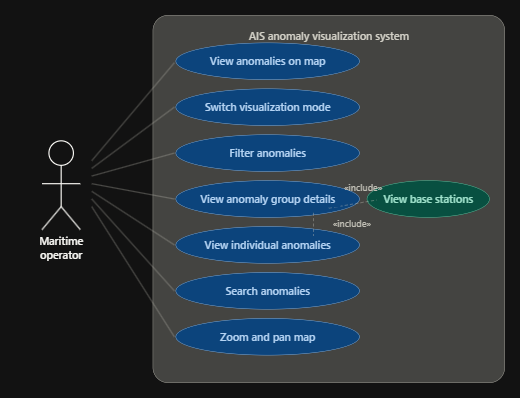
\includegraphics[width=0.95\textwidth,height=0.7\textheight,keepaspectratio]{Figures/Use_Case_Diagram.png}
    \caption[Use Case Diagram]{Use case diagram showing the expected interactions between a maritime operator and the system's core features}
    \label{fig:Use_Case_image}
\end{figure}

The use case diagram in Figure~\ref{fig:Use_Case_image} illustrates the expected user experience for a maritime operator. It showcases the core capabilities delivered by the system, allowing an operator to view anomalies, switch between different visualization layers, and access specific information regarding individual anomalies and anomaly groups.

\subsection{Package Diagram}

% SUGGESTION: replace with an updated package-diagram image if the directory structure changed.
\begin{figure}[H]
    \centering
    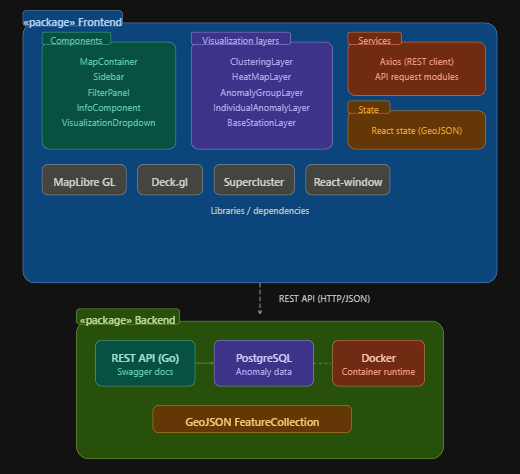
\includegraphics[width=0.95\textwidth,height=0.7\textheight,keepaspectratio]{Figures/Package_Diagram.png}
    \caption[Package Diagram]{Package diagram showing the modular directory structure of the frontend repository}
    \label{fig:Package_Diagram_image}
\end{figure}

The package diagram in Figure~\ref{fig:Package_Diagram_image} outlines the modular directory structure used in the frontend repository. Files are put into folders related to their function, such as components being isolated within a dedicated component folder, with necessary subfolders. This aligns with standard React component patterns as described in ~\ref{sec:react_theory}.

%TODO might need to add more theory to be able to better explain directory and patterns. also update the diagram to include all packages.
%, ensuring the codebase remains modular and easily navigable.
% SUGGESTION (relocate evaluation — your call): the clause "ensuring the codebase remains modular and
% easily navigable" is an assessment, not an observation of the diagram. Consider moving that
% judgement to Discussion (Technical Solution / Code Quality) and keeping only the structural fact
% here. Also verify you have a Theory reference for React package structure if you want to cite it.


\subsection{Sequence Diagram (Data Flow)}

\begin{figure}[H]
    \centering
    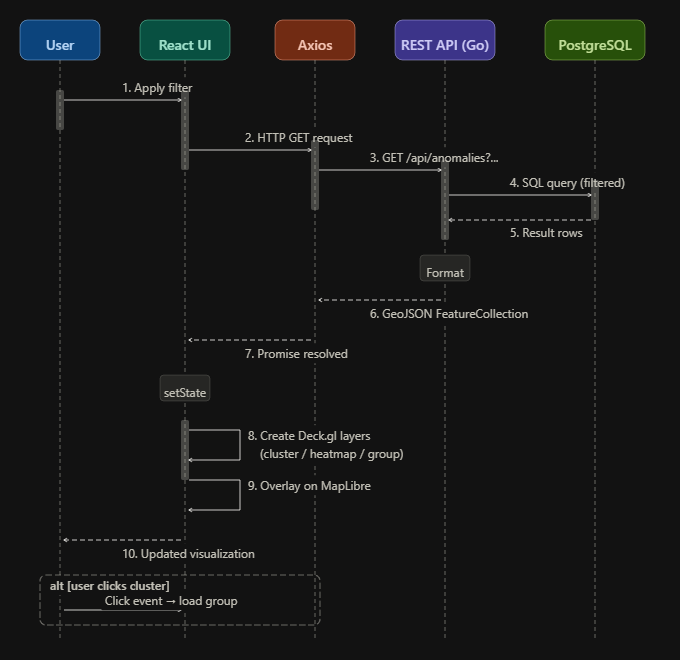
\includegraphics[width=0.95\textwidth,height=0.7\textheight,keepaspectratio]{Figures/Sequence_Diagram.png}
    \caption[Sequence Diagram]{Sequence diagram illustrating the data flow from a user filter action to an updated visualization layer}
    \label{fig:Sequence_Diagram_image}
\end{figure}

The sequence diagram in Figure~\ref{fig:Sequence_Diagram_image} maps the data flow from user interaction to visual state change. As illustrated in the image, if a user requests to apply a filter, an HTTP GET request is sent to an endpoint, which then queries the database. This then returns a GeoJSON FeatureCollection as a promise, and is then asynchronously accessed through React. This then creates the Deck.gl layer requested, and overlays it on the map, leading to an updated visualization for the end user.

\subsection{MapLibre}
% MOVED here from Visualization Results (4.6): MapLibre is architecture/runtime behaviour, mirroring
% its place under System Architecture in Method 3.2, not a visualization result.
MapLibre initializes itself upon application boot, in a bright style used for readability for users. After its initialization, it is responsible for interaction, in dragging and zooming the map. Interaction leads to states being updated that other parts of the program can use, such as clusters being updated through zooming, and map location. Visualization functionality is something MapLibre has, being able to natively visualize scatterplots and other layers. 
%TODO Start mentioning more about rational for choosing diffrent tools in method outside of them being suggested talking maybe about testing them before choosing.
%This was not chosen as a valid approach of visualization in the project, due to the high amount of data required to be visualized, which Deck.gl is specialized for.
% SUGGESTION (your call): the last sentence (why MapLibre was not used for visualization) is design
% rationale that may fit better in Method 3.2 (System Architecture / MapLibre) than in Results.

\section{Frontend}
\label{sec:results_frontend}
The resulting frontend of the project was created following the method in Section~\ref{sec:design_process}. Figure~\ref{fig:frontend_result_image} shows the finished frontend.

\begin{figure}[H]
    \centering
    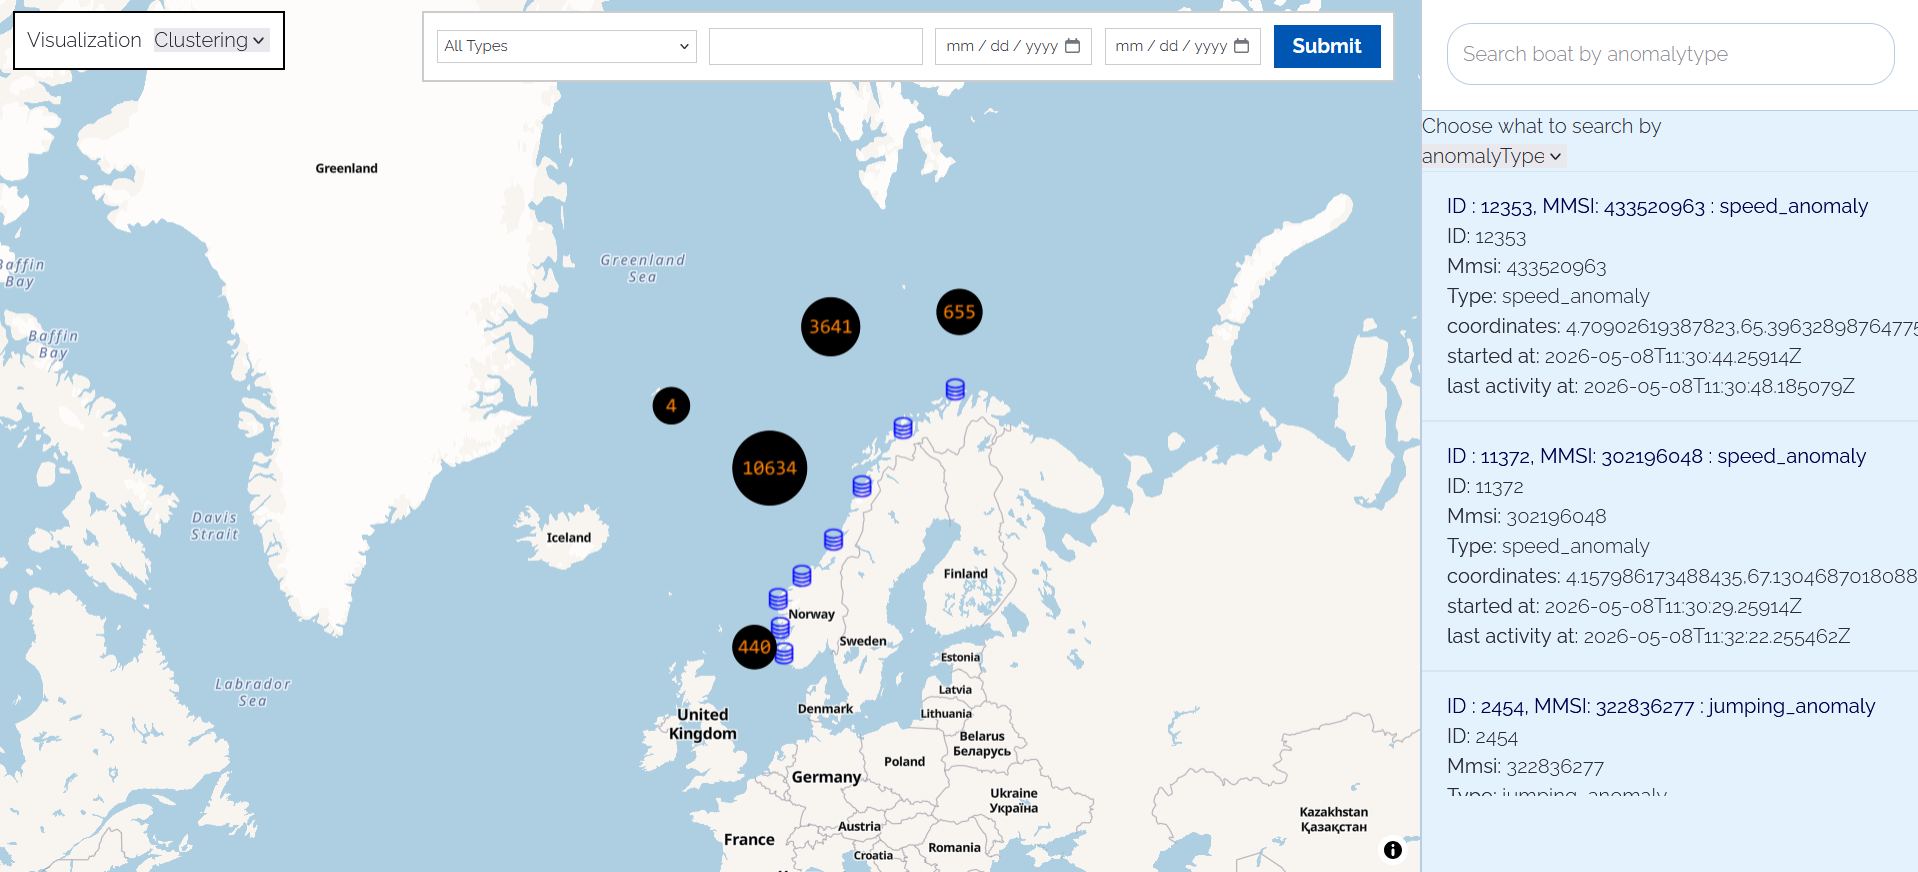
\includegraphics[width=0.95\textwidth,height=0.7\textheight,keepaspectratio]{Figures/full_application_image.png}
    \caption[Frontend application]{The completed single-page application showing the map view with visualization overlay, sidebar, and filter component}
    \label{fig:frontend_result_image}
\end{figure}

A singular page was created for the application, being the only page needed for all functionality. As shown in Figure~\ref{fig:frontend_result_image}, the user interface is made up of multiple parts. The base map takes up the center of the application, with visualization overlaid on top of the map.

Components such as a sidebar on the top right contain the entire dataset, allowing for searching of anomalies based on type or MMSI. 
A visualization dropdown menu allows switching between the two main visualization modes. 
On the top middle of the page is a filtering component, allowing users to change the displayed dataset by filtering on anomaly type, date range, and MMSI.
% SUGGESTION (4.4, wireframe link — you write the sentence(s)): add a link from the final UI back to
% the wireframes in Method 3.3. State whether the layout follows each wireframe (main page, date
% picker, filter) or diverged — e.g. the filter being moved to the top middle after customer
% feedback. Divergence-with-reason scores higher than "it matches", because it shows the design
% process fed real decisions.
%TODO add info since it wasa decided that the filter was moved to the top and after multiple visualization methods were added the top left has a permanent area for swapping betting clustering and heat maps. Also compared to the filter componenent it is wide to reduce clutter on the main page compared to the old filter in wireframe which had multiple fields for custom values as well as expandable lists for filtering. The final system became simpler with it only including type, mmsi and start and end date. While the sidebare stayed mostly the same however it now covers the whole right side. top to bottom. The ship info card stayed mostly the same with just a new button, which can show the anomalies in the group. Which was requested by the customer.

\section{Backend and Data Handling}
\label{sec:results_backend_and_data}
The backend, described in Section~\ref{sec:backend_and_data_flow_method}, was developed by the customer and provided as part of the project infrastructure. It exposes a REST API used by the frontend to retrieve anomaly data. Anomaly data is stored as a GeoJSON FeatureCollection, with each feature representing a single anomaly group.
\begin{figure}[H]
    \centering
    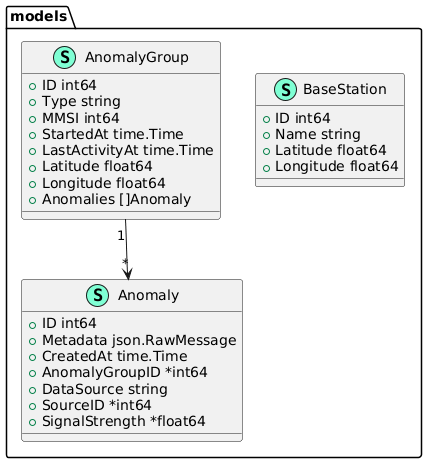
\includegraphics[width=0.54\textwidth,height=0.4\textheight,keepaspectratio]{Figures/db_models.png}
    \caption[Database model diagram]{Database model diagram showing the relationship between anomaly groups and individual anomalies}
    \label{fig:databse_model_diagram_image}
\end{figure}

\begin{figure}[H]
    \centering
    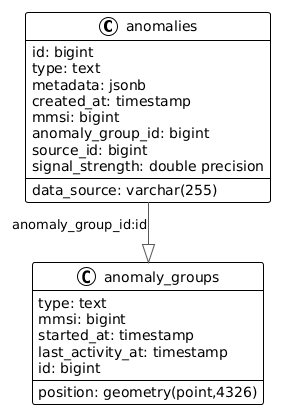
\includegraphics[width=0.54\textwidth,height=0.4\textheight,keepaspectratio]{Figures/db_result.png}
    \caption[Database schema]{Database schema showing table structure, field definitions, and data types}
    \label{fig:database_schema_image}
\end{figure}

Figures~\ref{fig:databse_model_diagram_image} and~\ref{fig:database_schema_image} show the backend database structure. An anomaly group contains anomalies, where the anomaly group itself has the start time and last activity time, sourced from the first instance of an anomaly being created in a group. Anomalies themselves have signal strength and their own data, with the group containing general data related to the group such as the general area of the anomalies, represented as location. 

The anomalies and anomaly groups are generated by the Docker backend, with the amount of anomalies set through a configuration file. Specific commands to generate anomalies and build the database are used, leading to a database filled with an amount of points set by the developer. The Docker backend running allows for the frontend to send requests to API endpoints to request data, while the frontend itself runs through localhost.

\subsection{GeoJSON Data Structure}

The final GeoJSON structure is shown in Figure~\ref{fig:geoJSON-result_image}.
\begin{figure}[H]
    \centering
    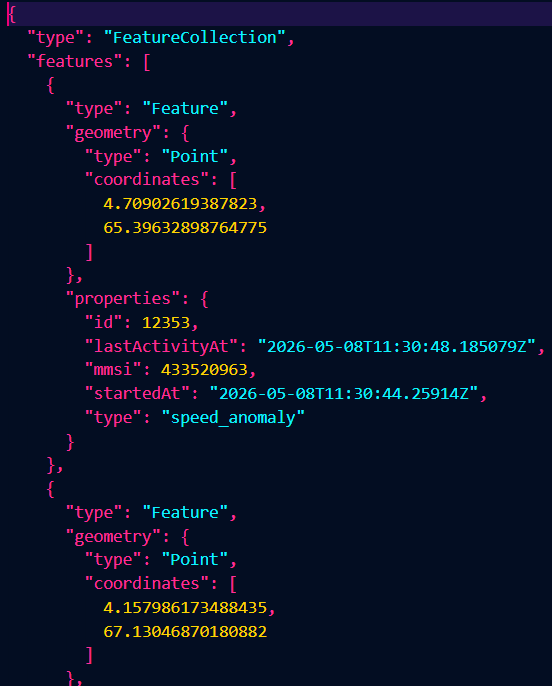
\includegraphics[width=0.54\textwidth,height=0.4\textheight,keepaspectratio]{Figures/geoJSON-result.png}
    \caption[GeoJSON FeatureCollection structure]{Example GeoJSON FeatureCollection returned by the backend API, with anomaly groups as individual features}
    \label{fig:geoJSON-result_image}
\end{figure}
Anomaly data is completely integrated in a FeatureCollection, with the individual features being anomaly groups. These features are individually processed in the frontend, as a dataset, through Deck.gl.

\subsection{Backend Query and Response Behaviour}
Figure~\ref{fig:swagger-result_image} showcases an API endpoint, created as a master query allowing for filtered requests on all relevant variables.
% SUGGESTION (own-contribution — you write it): the master query is one of your strongest own
% contributions. Name the parameters it accepts (e.g. anomaly type, MMSI, time range) and what a
% typical response contains, and bridge to Method 3.4 (Section~\ref{sec:backend_and_data_flow_method}).
% Make the boundary explicit: backend infrastructure was the customer's, this endpoint was the group's.
%TODO anomaly type, MMSI, time range were all included in the master query, this was a contribution to backend infrastructure the customer provided. Creating a new endpoint which returns all the anomaly groups with those variables. which includes all anomalies which includes base stations and signal strength within. Unsure if i should mention all that.

\begin{figure}[H]
    \centering
    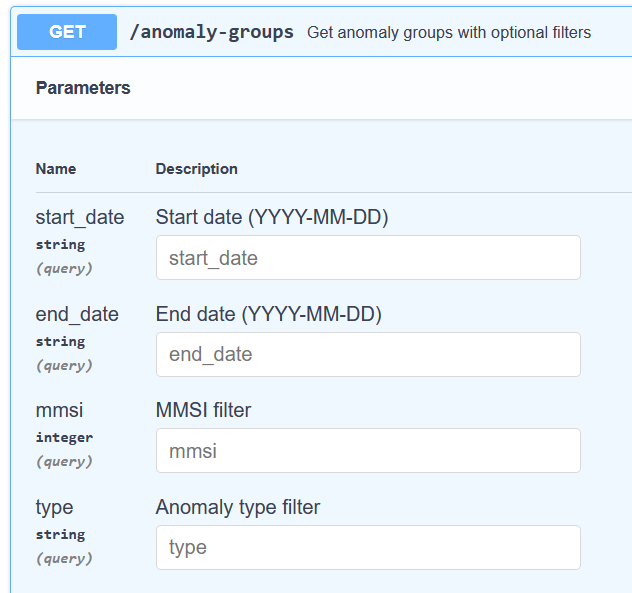
\includegraphics[width=0.54\textwidth,height=0.4\textheight,keepaspectratio]{Figures/swagger_api.png}
    \caption[Swagger API endpoint]{Swagger UI showing the master query endpoint with all available filter parameters}
    \label{fig:swagger-result_image}
\end{figure}
General endpoints for retrieving all anomaly data, as well as filtered datasets, are implemented. Requesting filtered data leads to the base dataset changing to contain the new data, while in other cases such as the sidebar having its own data variable to not change the main map data through search.

\section{Visualization Results}
\label{sec:results_visualization}
All visualization methods described in the Method chapter were implemented in the final system. The system includes clustering, heat map, base station, anomaly group, and individual anomaly visualization. Additional proposed features were not implemented.

\subsection{Clustering Visualization}
The clustering visualization was implemented as described in Section~\ref{sec:clustering_method}. The clustering approach uses Supercluster.js to calculate clusters through proximity based on radius and zoom level (Section~\ref{sec:supercluster}). This approach produces grouped anomaly points, with numeric labels indicating the number of anomalies in each cluster, as shown in Figure~\ref{fig:clustering_result_image}.
\begin{figure}[H]
    \centering
    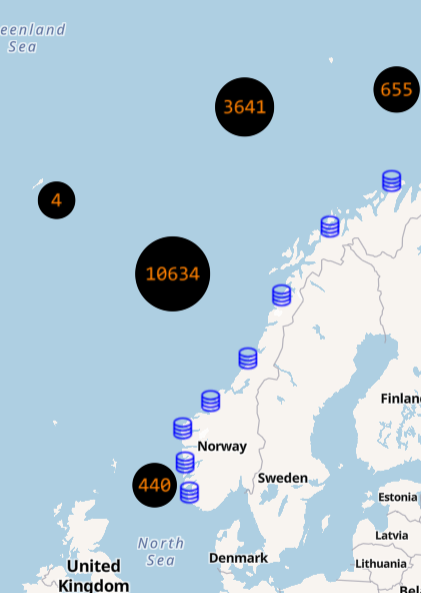
\includegraphics[width=0.4\textwidth,height=0.35\textheight,keepaspectratio]{Figures/clustering-result.png}
    \caption[Clustering visualization result]{Clustering visualization showing anomaly groups aggregated by proximity, with numeric labels indicating the group count per cluster}
    \label{fig:clustering_result_image}
\end{figure}
Clusters are calculated through the use of a radius that computes the amount of points inside a circle of a defined radius, in the case of the project being 40 pixels. Points inside the pixel radius are aggregated, and shown as a single point. A higher density of points in a cluster leads to that cluster being shown as larger on the map. Recalculation of clusters happens when zooming and dragging is done in the application, where clusters are divided into smaller parts due to points increasing in distance, moving outside of the defined radius.
% SUGGESTION (Method/Results bleed + figure-specific — your call): this paragraph re-derives the
% 40-pixel aggregation mechanism, which is really Method 3.5 content. Consider moving the mechanism to
% Method and replacing it here with what YOUR screenshot actually shows: which region, which zoom
% level, where the largest cluster sits and roughly how many anomalies it holds. The clustering
% performance effect is reported in Section~\ref{sec:effect_of_clustering_results}.
%TODO Use the image like suggested to show how it works now.


\subsection{Heat Map Visualization}
The system includes a heat map visualization layer. The heat map is implemented as in Section~\ref{sec:Heat_Map_method}. An example of the implemented heat map visualization is shown in Figure~\ref{fig:heatmap_result_image}.
\begin{figure}[H]
    \centering
    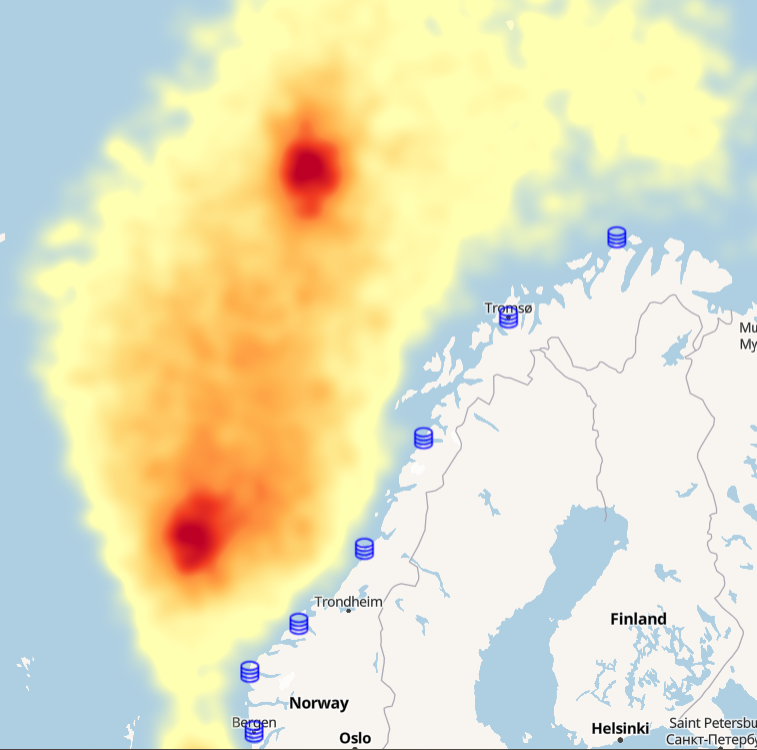
\includegraphics[width=0.54\textwidth,height=0.35\textheight,keepaspectratio]{Figures/heatmap-result.png}
    \caption[Heat map visualization result]{Heat map visualization showing anomaly density across the dataset, with warmer colors indicating higher concentrations}
    \label{fig:heatmap_result_image}
\end{figure}
Color is generated through calculating the sum of points inside a radius of 40 pixels, meaning points inside a circle are calculated as a sum, leading to higher density of points being weighted more \parencite{deckgl_official_site}. 
The resulting heat map layer allows for zoom and drag operations to change the heat map view dynamically, with zoomed in levels having less dense representation, while zoomed out levels lead to higher aggregates per pixel radius, and denser representation overall.
% SUGGESTION (Method/Results bleed + figure-specific — your call): the "sum of points inside a
% 40-pixel radius" sentence is mechanism (Method 3.5). For the result, describe what YOUR figure
% shows — name where the hot spots actually appear (e.g. "the highest concentration appears along
% the southern coast near X") rather than the generic "warmer = denser".
%TODO Same thing as clustering.

\subsection{Base Station Visualization}
A base station layer is part of the application, implemented as mentioned in Section~\ref{sec:base_station}. The base station layer is visualized through blue icons in Figure~\ref{fig:base_station_result_image}. The base station layer itself is persistent, meaning that it is a visualization layer that will always be present in the app, even if other methods of visualizing the data points are changed. 
\begin{figure}[H]
    \centering
    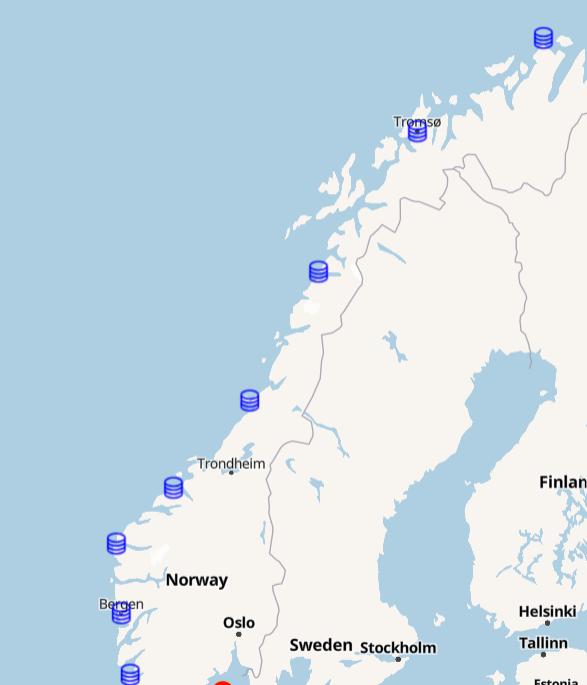
\includegraphics[width=0.4\textwidth,height=0.2\textheight,keepaspectratio]{Figures/Base-station-view.png}
    \caption[Base station layer]{Base station layer showing fixed AIS receiver locations as blue icons, providing persistent geographic reference points on the map}
    \label{fig:base_station_result_image}
\end{figure}
Base stations are linked to anomalies through backend data representing transmissions from individual anomalies. This is then used in other layers to connect base stations to anomalies through signal strength. The base station data itself will never change in position, as they are static points on the map. This provides persistent reference in relation to anomaly and transmitted base station, and helps end users visually observing the distance between anomaly cluster and base station, leading to visual feedback on the spatial relationship between anomalies and base stations.
% SUGGESTION (relocate evaluation — your call): "helps end users visually observing the distance...
% leading to visual feedback on the spatial relationship" is an assessment of usefulness, not an
% observation of the layer. Consider keeping the factual link (base stations are static reference
% points) here and moving the usefulness claim to Discussion.
%TODO Evaluations need to be moved


\subsection{Anomaly Group Visualization}
The anomaly group visualization is shown in Figure~\ref{fig:anomaly_group_result_image}.
\begin{figure}[H]
    \centering
    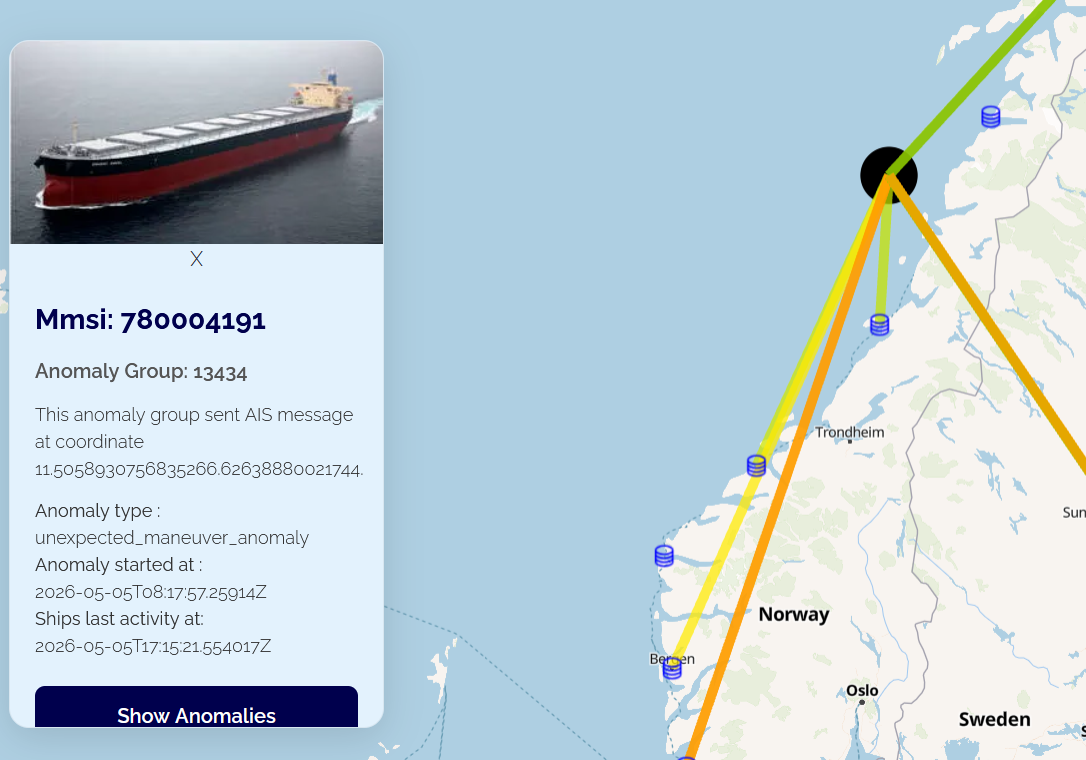
\includegraphics[width=0.8\textwidth,height=0.6\textheight,keepaspectratio]{Figures/anomaly-group-layer-result.png}
    \caption[Anomaly group layer]{Anomaly group layer showing signal strength lines connecting individual anomalies to nearby base stations and satellites}
    \label{fig:anomaly_group_result_image}
\end{figure}

The layer shows an info component for the current group, with coordinates, start date, and anomaly type. Signal strength is visualized through lines, connecting the individual anomalies inside the group to the base stations shown in the picture as blue symbols. The info component allows for users to show anomalies inside the group, through button press on the component, leading to the visualization being changed to the individual anomaly visualization. 


\subsection{Individual Anomaly Visualization}
Individual anomalies are shown as a scatter plot (Section~\ref{sec:scatter_plot}). The visualization shows the points colored based on signal strength, from red to green. This is done through the signal strength value being normalized from 0 to 1, in the database.
% SUGGESTION (Method/Results bleed — your call): "normalized from 0 to 1 in the database" is an
% implementation detail that fits better in Method 3.5. Results can simply state that points are
% coloured from red to green by signal strength.
%TODO Fix this
\begin{figure}[H]
    \centering
    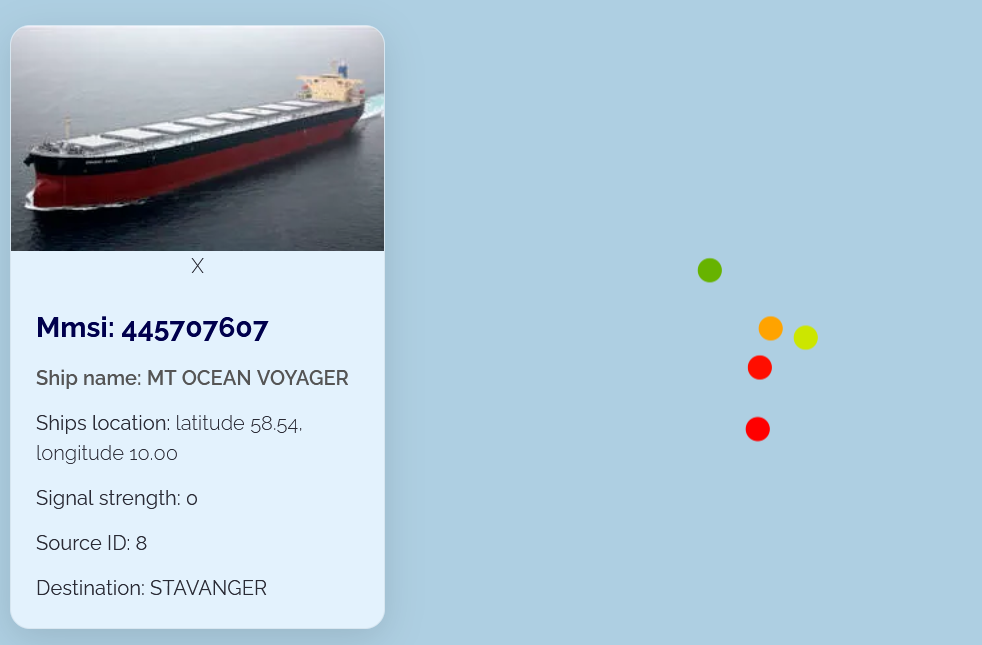
\includegraphics[width=0.54\textwidth,height=0.4\textheight,keepaspectratio]{Figures/individual_anomaly_layer_result.png}
    \caption[Individual anomaly layer]{Individual anomaly layer displaying anomalies as a scatter plot, colored from red to green based on signal strength}
    \label{fig:individual_anomaly_result_image}
\end{figure}
Figure~\ref{fig:individual_anomaly_result_image} shows the completed layer. Anomalies are correctly colored through the signal strength variable, with an info component being shown for an anomaly, through clicking on it. The info component illustrates features of the anomaly, like its direction, name, and MMSI.

% SUGGESTION (4.7 — mirrors Method 3.6;
% YOU still need to: add the screenshots (filter panel, a before/after of the dataset changing, the
% date picker, the satellite layer on click) and expand each description in your own words.
\section{Filter and Interaction}
\label{sec:results_filter_and_interaction}
This section presents the delivered filtering and interaction features, implemented as described in Section~\ref{sec:filter_and_interaction_method}.

\subsection{Filter System}
The filter system allows the rendered dataset to be narrowed by anomaly type, MMSI, and last activity date.
% SUGGESTION (you write/expand): add a screenshot of the filter panel (with a Figure ref) and a
% before/after pair showing the map dataset changing when a filter is applied. State the available
% parameters explicitly.

\subsection{Temporal Filtering}
A date-time range selector allows the visualization to be restricted to a chosen time period.
% SUGGESTION (you write/expand): add a screenshot of the date picker (Figure ref) and describe what
% the user sees when a range is applied.

\subsection{Satellite Visualization}
Satellite connections are displayed as a layer that appears only when a data point is clicked. 
% SUGGESTION (you write/expand): add a screenshot of the satellite layer appearing on click (Figure
% ref) and confirm exactly what triggers it.

\subsection{Interactive Components}
The interface provides interactive controls for selecting filter values.
% SUGGESTION (you write/expand): name the actual controls (e.g. pop-up calendar for dates, dropdown
% for anomaly type, numeric input for MMSI) and optionally add a screenshot.


\section{Testing and Performance}
\label{sec:results_testing}

Testing was done manually, as mentioned in Section~\ref{sec:testing_method}. Console logging and observation based testing was used, to ensure all features work, with performance testing being done through use of the application.
% SUGGESTION (4.8, testing findings — you write it): Method 3.7 has three subsections (Backend API,
% Frontend, Performance methodology) but this produces ~2 sentences of result. Add findings that
% mirror it: (1) a short list of features validated manually (layer switching, filter combinations,
% search, click/info interactions, date range); (2) what the Swagger API testing confirmed (endpoints
% return correct filtered data); (3) bugs found AND fixed during testing (e.g. the cluster-
% recalculation issue mentioned in Method). "Found and fixed" items show the testing did something.

The performance of the system has been observed through rigorous use of the application itself and logging individual parts. Each visualization type was observed at different zoom levels and areas of the map.
% SUGGESTION (de-subjectify — your call): "rigorous" is a subjective qualifier. Consider replacing it
% with what was actually done (which views, which zoom levels, roughly how many runs), and add the
% test hardware (GPU) and dataset sizes so the performance observations below have context.
%TODO Most tests were done with the default zoom with 2-3 refreshes of the website. However for the features that tested clicking of data points they were tested for usually just 2 points to make sure it worked on different points. The hardware utilized was just two labtops utilized by the group for school work. The main data size utilised was 10k points of data, however when testing we usually went up to 100k or 1 million data points. utilizing configs when starting up the backend which creates more template data for more points. The website always rendered data within a second of the request to the backend with most of the time used for sending the request and getting a response. Remaining within a responsive range for the website. By testing was also how we realised we needed a master query to make sure data was queryed all at once and not filtered on the frontend cause of the efficency on the backend.
% Need to get the actual number and some goes in the other subsection

\subsection{Rendering Performance}

The rendering performance is responsive, but will vary based on graphics processing speed of differing computers (Section~\ref{sec:hardware_acceleration}). Rendering happens first with the base map, then with data points, with the other user interface parts appearing with the map. Different visualization methods have different performance, with clustering being faster than heat maps in all cases.
% SUGGESTION (quantify — you write it): add approximate figures if available (dataset sizes tested,
% GPU used, rough layer-switch latency).

\subsection{Effect of Clustering on Performance}
\label{sec:effect_of_clustering_results}

Clustering had a profound effect on the speed of the application, where rendering a scatterplot natively, with over one hundred thousand data points, proved very inefficient. Clustering renders fewer data points, while the same data remains on the actual map. Due to data points being rendered as they are in view, clustering leads to fewer data points being shown while zoomed out, with zooming in showing more data points, while still not being cluttered as a normal scatterplot would be.
% SUGGESTION (quantify — highest-leverage fix, you write it): "profound effect" / "very inefficient"
% are judgments with no number behind them. Replace with a concrete observation you can state even
% from informal testing, e.g. "the plain scatter plot became unresponsive above approximately N
% points, while the clustered view remained interactive." Add the point counts rendered with vs
% without clustering at a given zoom if you have them; move any remaining judgment to Discussion.
%TODO do some actual test on the actual speed of the loading.

\subsection{System Responsiveness}

Responsiveness of the system is observed to be at a satisfactory level, although some operations cost more than others, such as going from a clustered view to an anomaly group view, with signal strength lines being computed, causes some slowdown, but remains responsive after the layer is changed. Other parts of the system like filtering and changing of layers are responsive, and change as soon as input is submitted. The slowest layer is heat maps, as changing zoom or moving around the map, causes it to recalculate the weight of each area. The heat map itself is as responsive as Deck.gl implemented it, leading to no considerable performance gains to be doable, outside of trying to implement a clustered heat map in some way.
% SUGGESTION (relocate evaluation + quantify — your call): "satisfactory level" and "no considerable
% performance gains to be doable" are judgments → move to Discussion. Here, state observed behaviour
% only, and add approximate wait times for the slower operations (e.g. the clustered to anomaly-group
% switch) if you have them.

\section{Customer Feedback}
\label{sec:customer_feedback}

Feedback was collected from two sources through the process described in Section~\ref{sec:user_feedback}: the product owner at Kystverket, and an internal user who works with the AIS analysis system that is closely related to this project.

\subsection{Product Owner Evaluation}

The product owner evaluated the delivered features across four areas: clustering, signal strength visualization, heat map, and the solution as a whole.

\subsubsection{Clustering}

The clustering visualization was assessed positively because it helped provide a proper overview over a large amount of data without the visual clutter. The product owner also noted that clustering is already utilized by other large data systems at Kystverket, however it has not yet been applied to the AIS anomaly monitoring. A suggestion that was given for further development was to be able to display the types and counts of anomalies within each cluster. This would allow operators to assess if further exploring a cluster is worthwhile quickly.

\subsubsection{Signal Strength}

The signal strength visualization was described as a concept they were very interested in. The product owner noted that low signal strength between a vessel and a base station is an error in AIS messages that causes the creation of anomaly messages. Other systems they utilise for signal strength take longer to find the data and do not visualise it properly, increasing the time to analyse anomaly groups and the time complexity for the operator. The delivered solution was assessed as effective both at the macro level, where lines from anomaly groups to base stations are visible while zoomed out, and at the micro level, where individual signal strength values are visible when zoomed in. A suggestion was given to extend the visualization to include additional data like signal strength before and after an anomaly occurs, however this would require additional data from Kystverket.

\subsubsection{Heat Map}

The heat map was assessed to be a useful tool that complements clustering. This was because clustering only shows volume through numbers for large areas and requires zooming in to find areas with large amounts of points, while the heat map is valuable since it allows identification of all the hot spots on a large map at a zoomed-out level without requiring additional work from the user.

\subsubsection{General Solution}

The overall solution was evaluated positively for its features like toggling between visualization types, filtering by anomaly type, and the ability to drill down to the individual anomaly level. The product owner also noted that reimplementing anomaly group and base station views was necessary for the signal strength concept to provide value, even though those views already exist in Kystverket's current system.

\subsection{Internal User Feedback}

An internal user of Kystverket's existing AIS analysis system provided additional suggestions for further development.

\begin{itemize}
  \item Normalizing the heat map against vessel traffic density in
    each area, so that the visualization reflects where anomalies are
    overrepresented rather than where traffic volume is highest.
  \item Extending signal strength visualization to cover all position
    reports from a vessel, not only those linked to anomalies, to
    provide a more complete picture of signal quality over time.
  \item Disabling clustering at low data densities where
    consolidation removes useful detail from the view.
  \item Adding aggregated per-vessel statistics to support long-term
    credibility assessment of individual ships.
  \item Displaying anomaly frequency graphs over time to reveal how
    the situation develops hourly or daily.
\end{itemize}

\section{Project Outcome}

The final project outcome was influenced both by the original project outline and by scope changes introduced throughout development. The implemented system follows the main goals of the original project outline, but has different features implemented as a result of the change of scope.

\subsection{Scope Changes During Development}

During development, and from the start of the project, the project differed in scope from the project outline in subtle ways. All visualization methods that the group worked on were in the project outline, but during the project itself the focus of the application became testing new concepts, such as signal strength visualization, through lines going from anomaly to base station/satellite came later during the project lifecycle. Features such as report generation were not mentioned later in meetings or as a feature request, rather other features were chosen for concept testing. As a result of the scope never being locked down during the project, the customer gave requests on what at a certain point in time would be good to implement to see if value could be gotten in a full implementation in their own software.
% SUGGESTION (relocate evaluation — your call): "As a result of the scope never being locked down..."
% is a judgment that Discussion (Project Execution) already covers. Consider keeping only WHAT changed
% here (features added/removed) and moving the assessment to Discussion.

% Probably create a table for scope here and then for deliverd vs planned

\subsection{Delivered vs Planned Features}

Almost all planned features from the project outline and through meetings were implemented, some being seen as extra features later in development by the customer. A report generating system and satellite orbit visualization feature were not delivered. However satellites themselves were implemented and shown as connected to anomalies through a signal strength line in the anomaly group layer, showing its position at the time of data transmission. The overall delivered features implement the majority of the project outline's features, while also implementing the requested features from the customer.
% SUGGESTION (table + måloppnåelse honesty — you write it): replace this paragraph with a table —
% Feature | Status (Implemented / Partial / Not implemented) | Notes — listing EVERY objective from
% the Introduction, including shortfalls. The audit flags three to list honestly: Temporal Analysis
% "forward and backward in time" (Intro) -> delivered only a date-range filter = PARTIAL; hexagonal
% binning (project brief) -> NOT implemented; satellite orbit plotting -> NOT implemented. A sensor
% cross-checking the Introduction against Results will catch omissions, so list them.


%TODO Move this to the other one.
% SUGGESTION (relocate whole section to Discussion — your call; Discussion lives in 07Discussion.tex,
% out of my current scope): this entire section is comparative EVALUATION, not a result. Consider
% moving it wholesale into Discussion. If it stays here, it caps how factual the Results chapter reads.
\section{Comparison to Customer's Tools}

As the resulting application is testing concepts for the customer, a direct comparison yields little value, as the customer themselves mentioned that the currently in use tools are superior in their core functionality. However as the currently implemented application is testing new visualization methods and features, this then brings value to the customer to test if their already in use software, or software they are to make themselves, should have these features. As a result the software created for the project is better in the specifics of testing new concepts.

%=====================================================================